\documentclass[../main.tex]{subfiles}
\begin{document}
\chapter{Central Forces}
An important class of potentials depend only on the distance to some origin.
For example in \cref{gravity}, we saw that the force one one mass depends on its radial distance to another mass, so, if we treat the other mass s the origin, the force on the first particle depends only on its distance $r$ to that origin.
Similarly, in \cref{electricForces}, we saw that the force on one charge depends on its radial distance to another charge.

We can therefore express such potentials $V$ as a function of the radial distance:
\[
  V(\vec{x}) = V(|\vec{x}|) = V(r) \text{ where $r = |\vec{x}|$}
\]
The conservative force (\cref{conservativeForce}) associated with such a potential therefore points towards, or away from, the origin:
\begin{align}
  \vec{F} &= - \nabla V(r) \nonumber \\
          &= - \deriv{V}{r} \nabla r \text{ using the chain rule} \nonumber \\
          &= - \deriv{V}{r} \uvec{x} \text{ as $\nabla r = \frac{\vec{x}}{r}$ from \cref{gravity}} \label{radialForce}
\end{align}
which either points towards or away from the origin in the direction of $\uvec{x}$.
\begin{remark}[Notation]
  Sometimes we will denote $\frac{\vec{x}}{r}$ as $\uvec{r}$ or $\vec{e}_r$ instead of $\uvec{x}$.
\end{remark}
\section{Conservation of Angular Momentum}
\label{angularMomentum}
The most important fact about \textit{central potentials} is that \textit{angular momentum} is conserved.
\begin{definition}[Angular Momentum]
  The \textit{angular momentum} $\vec{L}$ of a particle of mass $m$ at $\vec{x}$ relative to its centre of rotation is defined to be:
  \[
    \vec{L} = m \vec{x} \times \dot{\vec{x}} = \vec{x} \times \vec{p}
  \]
\end{definition}
\begin{remark}
  $\vec{L}$ is defined relative to an origin, here we are setting the origin at $\vec{x} = \vec{0}$, however, we will generalise later.
\end{remark}
Note that the angular momentum is orthogonal to both position and momentum/velocity.
\begin{center}
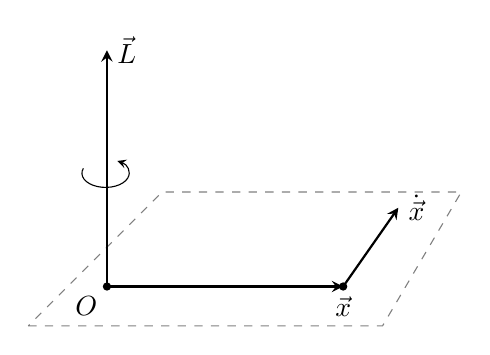
\begin{tikzpicture}[>=stealth]
  \draw[gray, dashed] (-1,-0.5) -- (3.5, -0.5) -- (4.5, 1.2) -- (0.7, 1.2) -- cycle;
  \fill (0, 0) circle (1.5pt) node[below left] {$O$};
  \draw[thick,->] (0,0) -- (3,0) node[below] {$\vec{x}$};
  \fill (3, 0) circle (1.5pt);
  \draw[thick,->] (3,0) -- (3.7,1) node[right] {$\dot{\vec{x}}$};
  \draw[thick,->] (0,0) -- (0,3) node[right] {$\vec{L}$};
  \draw[->, yscale=0.6] (-0.3,2.5) arc [start angle=-200,end angle=60,radius=0.3];
\end{tikzpicture}
\end{center}
For a general force $\vec{F}$:
\begin{align*}
  \deriv{\vec{L}}{t} &= m \deriv{}{t}(\vec{x} \times \dot{\vec{x}}) \\
                     &= m(\cancelto{\vec{0}}{\dot{\vec{x}} \times \dot{\vec{x}}} + \vec{x} \times \ddot{\vec{x}}) \\
                     &= \vec{x} \times (m \ddot{\vec{x}}) \\
                     &= \vec{x} \times \vec{F}
\end{align*}
We define the \textit{torque} to be $\vec{G} \equiv \vec{x} \times \vec{F}$.
\begin{remark}
  $\deriv{\vec{L}}{t} = \vec{G}$ is analogous to Newton's 2nd Law (\cref{newton2}), but for angular momentum.
\end{remark}
\label{angularConserved}
For a central force, $\vec{F} \parallel \vec{x} \implies \vec{x} \times \vec{F} = \vec{0} \implies \deriv{\vec{L}}{t} = 0$ and thus angular momentum is conserved by central forces.

Because $\vec{L}$ is a constant vector and obeys $\vec{L} \cdot \vec{x} = 0$ and $\vec{L} \cdot \dot{\vec{x}} = 0$, both the position and velocity are contained to a plane perpendicular to $\vec{L}$ and so 3D dynamics reduce to 2D dynamics on a plane.
\section{Polar Coordinates in the Plane}
\begin{definition}[Plane Polar Coordinates]
  Plane polar coordinates are defined by:
  \[
    x = r \cos \theta,\ y = r \sin \theta
  \]
  where $r \geq 0$ and $\theta$ can be restricted to $(0, 2\pi]$.
  We write the components in the order $(r, \theta)$.
\end{definition}
\begin{center}
\begin{tikzpicture}[>=stealth]
  \draw[->] (-0.5, 0) -- (3, 0) node[right] {$x$};
  \draw[->] (0, -0.5) -- (0, 3) node[above] {$y$};

  \draw[->, thick] (0, 0) -- (1.5, 1.5) node[below right] {$\vec{x}$} node[midway, above] {$r$};
  \draw (0.6,0) arc [start angle=0,end angle=45,radius=0.6] node[pos=0.7,right] {$\theta$};
  \fill (1.5, 1.5) circle (1.5pt);
  \draw[->] (1.5, 1.5) -- (1, 2) node[left] {$\uvec{\theta}$};
  \draw[->] (1.5, 1.5) -- (2, 2) node[right] {$\uvec{r}$};
\end{tikzpicture}
\end{center}
At each point, there is a local basis $\{\uvec{r}, \uvec{\theta}\}$ given in Cartesian coordinates by:
\[
  \uvec{r} = \begin{pmatrix}
  \cos \theta \\
  \sin \theta \\
  \end{pmatrix},\
  \uvec{\theta} = \begin{pmatrix}
  -\sin \theta \\
  \cos \theta \\
  \end{pmatrix}
\]
Recall from Vector Calculus that these vectors depend on position:
\[
  \deriv{\uvec{r}}{\theta} = \begin{pmatrix}
  -\sin \theta \\
  \cos \theta \\
  \end{pmatrix} = \uvec{\theta},\
  \deriv{\uvec{\theta}}{\theta} = \begin{pmatrix}
  -\cos \theta \\
  -\sin \theta \\
  \end{pmatrix}= -\uvec{r}
\]
We need to keep track of these changes when we write vector equations using polar coordinates.
We can write $\vec{x} = r \uvec{r}$ so we can differentiate to find $\ddot{\vec{x}}$:
\begin{align*}
  \dot{\vec{x}} &= \dot{r} \uvec{r} + r \dot{\uvec{r}} \\
                &= \dot{r} \uvec{r} + r \deriv{\uvec{r}}{\theta} \deriv{\theta}{t} \\
                &= \dot{r} \uvec{r} + r \dot{\theta} \uvec{\theta}
\end{align*}
$\dot{\theta}$ is often called the \textit{angular velocity}.

We can differentiate again to get $\ddot{\vec{x}}$:
\begin{align*}
  \ddot{\vec{x}} &= \ddot{r} \uvec{r} + \dot{r}\dot{\uvec{r}} + \dot{r} \dot{\theta} \uvec{\theta} + r(\ddot{\theta}\uvec{\theta} + \dot{\theta}\dot{\uvec{\theta}}) \\
                 &= \ddot{r} \uvec{r} + 2 \dot{r} \dot{\theta} \uvec{\theta} + r \ddot{\theta} \uvec{\theta} - r \dot{\theta}^2 \uvec{r} \\
                 &= (\ddot{r} - r \dot{\theta}^2)\uvec{r} + (r \ddot{\theta}  + 2\dot{r} \dot{\theta}) \uvec{\theta}
\end{align*}
\begin{example}[Circular Motion]
  Suppose we have circular motion at a constant angular velocity $\omega$.
  We then have $\dot{r} = 0,\ \ddot{r} = 0$ and $\dot{\theta} = \omega,\ \ddot{\theta} = 0$.
  Even though both $\ddot{r}$ and $\ddot{\theta}$ are 0, this does not mean that the particle is not accelerating as we see that:
  \[
    \ddot{\vec{x}} = (0 - r\omega^2)\uvec{r} + (r(0) + 2(0)(0))\uvec{\theta} =  -r \omega^2 \uvec{r}
  \]
  So we require an acceleration towards the origin and therefore a \textit{centripetal force} towards the origin.
  \begin{center}
  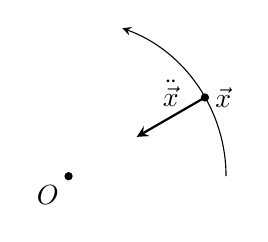
\begin{tikzpicture}[>=stealth]
    \fill (0, 0) circle (1.5pt) node[below left] {$O$};
    \draw[->] (2,0) arc [start angle=0,end angle=70,radius=2];
    \coordinate (X) at (1.732, 1);
    \draw[->, thick] (X) node[right] {$\vec{x}$} -- (0.866, 0.5) node[midway, above] {$\ddot{\vec{x}}$};
    \fill (X) circle (1.5pt);
  \end{tikzpicture}
  \end{center}
  If there was no such force, then the velocity of the particle would be constant and so it would just travel in a straight line.
\end{example}
To write Newton's second law for a central force, recall from \cref{radialForce} that $\vec{F} = -\deriv{V}{r}\uvec{r}$.
Combining this with the above, we have:
\[
  m\ddot{x} = m(\ddot{r} - r \dot{\theta}^2)\uvec{r} + m(r \ddot{\theta}  + 2\dot{r} \dot{\theta}) \uvec{\theta} = -\deriv{V}{r}\uvec{r}
\]
Since $\uvec{r}$ and $\uvec{\theta}$ form an orthonormal basis, we can equate the radial and angular components to yield:
\begin{align}
  \uvec{r}:&\ m(\ddot{r} - r \dot{\theta}^2) = -\deriv{V}{r} \label{eqnRadial} \\
  \uvec{\theta}:&\ r\ddot{\theta}  + 2\dot{r}\dot{\theta} = 0 \label{eqnAngular}
\end{align}
We can rewrite \cref{eqnAngular} as:
\begin{align}
  \frac{1}{r}\deriv{}{t}(r^2 \dot{\theta}) &= 0 \nonumber \\
  \implies r^2 \dot{\theta} &= \ell \text{ is constant} \label{rthetadot}
\end{align}
In fact, this is the magnitude of the angular momentum:
\begin{align*}
  \vec{L} = m \vec{x} \times \dot{\vec{x}} &= m r \uvec{r} \times(\dot{r} \uvec{r} + r \dot{\theta}\uvec{\theta}) \\
                                           &= m r \dot{r} \cancelto{\vec{0}}{\uvec{r} \times \uvec{r}} + mr^2 \dot{\theta} \uvec{r} \times \uvec{\theta} \\
                                           &= mr^2 \dot{\theta} \uvec{r} \times \uvec{\theta}
\end{align*}
Note that $\uvec{r}$ and $\uvec{\theta}$ are orthogonal unit vectors so their cross product is also a unit vector, thus:
\[
  |\vec{L}| = m r^2 \dot{\theta} = m \ell
\]
\begin{remark}
  We sometimes refer to $\ell$ as ``angular momentum'' despite it technically being angular momentum \textit{per unit mass}.
\end{remark}

To get rid of the $\theta$ dependence in \cref{eqnRadial}, we can substitute $\dot{\theta} = \ell/r^2$:
\begin{align*}
  m\left(\ddot{r} - r\frac{\ell^2}{r^4}\right) &= -\deriv{V}{r} \\
  m\ddot{r} &= - \deriv{V}{r} + \frac{m\ell^2}{r^3} \\
            &= -\deriv{}{r}\left(V + \frac{m\ell^2}{2r^2}\right) \\
            &= -\deriv{V_{\text{eff}}}{r}
\end{align*}
where $V_{\text{eff}} = V(r) + \frac{m\ell^2}{2r^2}$ is called the \textit{effective potential}.

So we have effectively reduced the problem in 2D plane polar coordinates down to a one dimensional problem.
This is all possible because of the conserved angular momentum.
\section{Effective Potential}
Consider $V(r) = -\frac{k}{r}$, i.e. an attractive $\frac{1}{r}$ potential (as seen for gravity in \cref{gravity}) so that:
\[
  V_{\text{eff}}(r) = -\frac{k}{r} + \frac{m\ell^2}{2r^2}
\]
We can plot the graph of this to analyse the motion in the radial direction:
\begin{center}
\begin{tikzpicture}[scale=1.13, >=stealth]
  \draw[->] (0, 0) -- (9, 0) node[right] {$r$};
  \draw[->] (0, -2) -- (0, 2) node[above] {$V_{\text{eff}}$};

  \node at (1.7, 1.5) {$\frac{m\ell^2}{2r^2}$ behaviour};
  \node at (7, -1) {$-\frac{k}{r}$ behaviour};

  \def\kconst{4.5}
  \def\mlconst{3}

  \clip (0,-2) rectangle (9,2);
  \draw[thick, domain=0.1:9, smooth, samples=100] plot (\x,{-\kconst/\x + \mlconst/(\x)^2});
  \draw[|-|, thick] (0, -0.1) -- (0.67, -0.1) node[midway, below] {\small B};
\end{tikzpicture}
\end{center}
Region $B$ above is known as the \textit{centrifugal barrier}.
In this region, the angular momentum prevents the particle from getting too close to the origin.

We can also derive the effective potential from the conserved energy:
\begin{align*}
  E &= \frac{1}{2} m \dot{\vec{x}} \cdot \dot{\vec{x}} + V(r) \\
    &= \frac{1}{2} m (\dot{r} \uvec{r} + r \dot{\theta} \uvec{\theta}) \cdot (\dot{r} \uvec{r} + r \dot{\theta} \uvec{\theta}) + V(r) \\
    &= \frac{1}{2} m (\dot{r}^2 + r^2 \dot{\theta}^2) + V(r) \text{ as $\uvec{r} \cdot \uvec{\theta} = 0$ and $|\uvec{r}| = |\uvec{\theta}| = 1$}\\
    &= \frac{1}{2} m \dot{r}^2 + \frac{1}{2} m r^2 \left(\frac{\ell}{r^2}\right)^2 + V(r) \\
    &= \frac{1}{2} m \dot{r}^2 + V(r) + \frac{m\ell^2}{2r^2} \\
    &= \frac{1}{2} m \dot{r}^2 + V_{\text{eff}}(r)
\end{align*}
Note that the centrifugal barrier $\frac{1}{2}m\dot{r}^2$ is the \textit{angular kinetic energy}.

For $V(r) = - \frac{k}{r}$, there are a range of motions that can occur depending on the conserved energy of the object:
\begin{center}
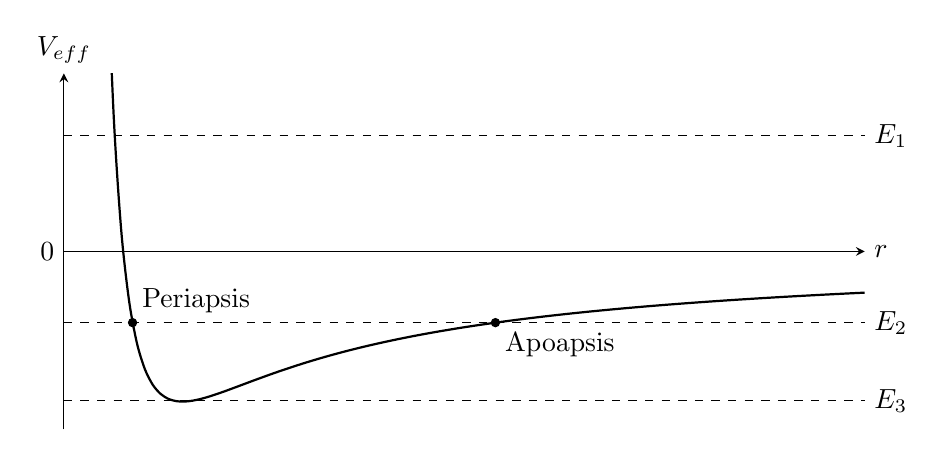
\begin{tikzpicture}[scale=1.13, >=stealth]
  \draw[->] (0, 0) node[left] {0} -- (9, 0) node[right] {$r$};
  \draw[->] (0, -2) -- (0, 2) node[above] {$V_{\text{eff}}$};

  \def\kconst{4.5}
  \def\mlconst{3}

  \draw[dashed] (0, 1.3) -- (9, 1.3) node[right] {$E_1$};
  \draw[dashed] (0, -0.8) -- (9, -0.8) node[right] {$E_2$};
  \draw[dashed] (0, -1.68) -- (9, -1.68) node[right] {$E_3$};

  \fill (0.772, -0.8) circle (1.5pt) node[above right] {Periapsis};
  \fill (4.85, -0.8) circle (1.5pt) node[below right] {Apoapsis};

  \clip (0,-2) rectangle (9,2);
  \draw[thick, domain=0.1:9, smooth, samples=100] plot (\x,{-\kconst/\x + \mlconst/(\x)^2});
\end{tikzpicture}
\end{center}
\textbf{Potential Motions}:
\label{potentialOrbitMotions}
\begin{itemize}
  \item When $E = E_1$, we get unbounded, \textit{hyperbolic} motion.
  \item When $E = E_2$, we get bounded, \textit{elliptic} motion.
    The point of closes approach is called the \textit{periapsis} and the farthest point is called the apoapsis.
  \item When $E = E_3$, we get bounded, \textit{circular} motion.
    This is a \textbf{stable} equilibrium point so the circular orbit is stable.
  \item When $E = 0$, we get unbounded, \textit{parabolic} motion.
\end{itemize}

Suppose instead that $V(r) = -\frac{k}{r^{n}}$ for $n > 2$
\begin{center}
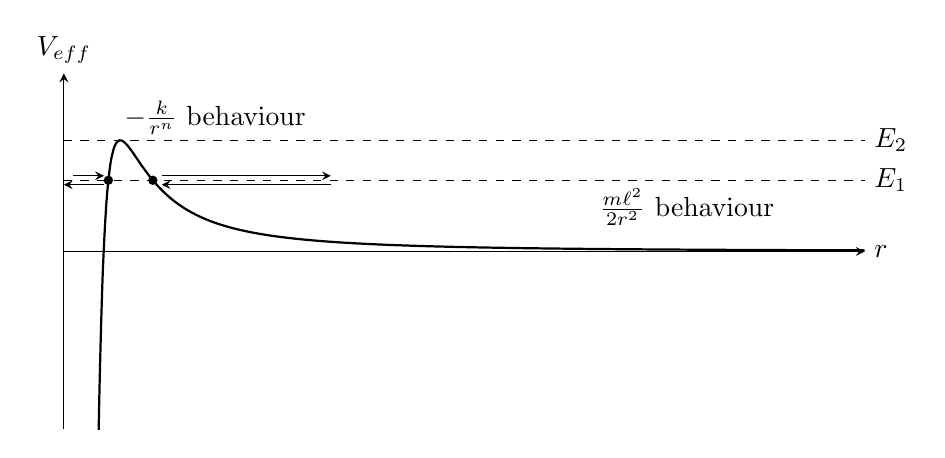
\begin{tikzpicture}[scale=1.13, >=stealth]
  \draw[->] (0, 0) -- (9, 0) node[right] {$r$};
  \draw[->] (0, -2) -- (0, 2) node[above] {$V_{\text{eff}}$};

  \def\kconst{0.2}
  \def\mlconst{1}

  \node at (1.7, 1.5) {$-\frac{k}{r^{n}}$ behaviour};
  \node at (7, 0.5) {$\frac{m\ell^2}{2r^2}$ behaviour};


  \draw[dashed] (0, 0.8) -- (9, 0.8) node[right] {$E_1$};
  \draw[->] (1.1, 0.85) -- (3, 0.85);
  \draw[<-] (1.1, 0.75) -- (3, 0.75);
  \fill (1, 0.8) circle (1.5pt);
  \fill (0.5, 0.8) circle (1.5pt);
  \draw[->] (0.1, 0.85) -- (0.45, 0.85);
  \draw[<-] (0, 0.75) -- (0.45, 0.75);
  \draw[dashed] (0, 1.25) -- (9, 1.25) node[right] {$E_2$};


  \clip (0,-2) rectangle (9,2);
  \draw[thick, domain=0.3:9, smooth, samples=200] plot (\x,{-\kconst/(\x)^4 + \mlconst/(\x)^2});
\end{tikzpicture}
\end{center}
\textbf{Potential Motions}
\begin{itemize}
  \item When $E = E_1$, either the particle comes in from a large $r$, ``bounces'' off the potential and then shoots off to $\infty$, or starts at a small $r$ and then ``bounces'' off the potential before falling in towards the object it is attracted towards.
  \item When $E = E_2$, we get a bounded circular orbit, however, unlike the $V(r) \propto \frac{1}{r}$ case, this is a \textbf{unstable} equilibrium point.
    So it is not a stable orbit so even a small force would cause either cause the object to fall towards the body it is orbiting, or cause it to drift off to $\infty$.
\end{itemize}
Therefore, if $V(r) = -\frac{k}{r^{n}}$ for $n > 2$, there are no stable bound orbits.
Gravity in a $d$-dimensional space satisfies $V \propto \frac{1}{r^{d - 2}}$ so circular orbits are only stable in $d < 4$ (which \textit{thankfully} includes $d = 3$).
\section{The Orbit Equation}
\subsection{General Orbit Equation}
Centuries of study of this problem have found that it is most convenient to work using the substitution $u = \frac{1}{r}$.

We currently have the equation:
\begin{align}
  &m\ddot{r} = -\deriv{V_{\text{eff}}}{r} = - \deriv{}{r}\left(V(r) + \frac{m\ell^2}{2r^2}\right) = - \deriv{V}{r} + \frac{m\ell^2}{r^3} \nonumber \\
  &\implies m\ddot{r} - \frac{m\ell^2}{r^3} = - \deriv{V}{r} = F(r) \label{orbitUntransformed}
\end{align}
which tells us $r$ as a function of time.
However, to study the shape of the orbit, we would like $r$, or in this case $u$, as a function of $\theta$.

Changing variables first from $r(t) \to r(\theta)$, we have:
\[
  \dot{r} = \deriv{r}{t} = \deriv{r}{\theta}\dot{\theta} = \deriv{r}{\theta} \frac{\ell}{r^2}  \\
\]
as $r^2 \dot{\theta} = \ell$ from \cref{rthetadot}.
Now using $r(\theta) = \frac{1}{u(\theta)}$.
\[
  \deriv{r}{\theta} = - \frac{1}{u^2} \deriv{u}{\theta} = -r^2 \deriv{u}{\theta} \implies \dot{r} = -\ell \deriv{u}{\theta}
\]
Taking the derivative with respect to $t$ again:
\[
  \ddot{r} = \deriv[2]{r}{t} = \deriv{}{t}\left(-\ell \deriv{u}{\theta}\right) = -\ell \deriv[2]{u}{\theta} \dot{\theta} = - \ell^2 u^2 \deriv[2]{u}{\theta}
\]
So under the change of variables, \cref{orbitUntransformed} becomes:
\begin{align*}
  &-\ell^2 m u^2 \deriv[2]{u}{\theta} - mu^3\ell^2 = F\left(\frac{1}{u}\right) \\
  &\implies \deriv[2]{u}{\theta} + u = - \frac{1}{m\ell^2 u^2}F\left(\frac{1}{u}\right)
\end{align*}
\subsection{Kepler Problem}
\label{keplerSection}
Since we are modeling the particle under gravity, let $V(r) = -\frac{km}{r}$ where $k = GM$ (as we saw in \cref{gravity}).
With this potential, this is called the \textit{Kepler problem}.
\[
  F(r) = -\deriv{V}{r} = - \frac{km}{r^2} \implies F\left(\frac{1}{u}\right) = -kmu^2
\]
Substituting this back into the differential equation, we have:
\[
  \deriv[2]{u}{\theta} + u = \frac{k}{\ell^2}
\]
This is the equation for a harmonic oscillator with a displaced centre so has solution:
\[
  u = A \cos(\theta - \theta_0) + \frac{k}{\ell^2}
\]
For arbitrary constants $A$ and $\theta_0$.
So $u$ is largest when $\theta = \theta_0$, and so $r$ is smallest there, i.e. the periapsis.
For convenience, choose axes on the plane such that $\theta_0 = 0$, so the periapsis will always lie on the line $\theta = 0$.
\begin{align*}
  u = \frac{1}{r} &= A\cos \theta + \frac{k}{\ell^2} \\
  r &= \frac{\ell^2}{\ell^2 A \cos \theta + k} \\
    &= \frac{\ell^2 / k}{(\ell^2 A/k) \cos \theta + 1}
\end{align*}
For convenience, we then define the constant $r_0 = \ell^2/k$ and redefine the arbitrary constant so that $e = \frac{\ell^2 A}{k}$.
The final solution is then:
\begin{equation}
  r = \frac{r_0}{e\cos \theta + 1} \label{keplerProblem}
\end{equation}
As we saw in IA Vectors and Matrices, this is the equation for a conic section in polar coordinates.
The constant $e$ is called the \textit{eccentricity} of the orbit/conic section.
\begin{remark}
  Planets in the solar system all have small $e$ so are almost circular.
  Mercury's orbit has $e \approx 0.2$ whereas Halley's comet has $e \approx 0.97$, which is \textit{almost} an unbounded orbit.
\end{remark}

\subsection{Orbit Trajectories}
\label{orbitTrajectories}
There are then four cases, corresponding to those in \cref{potentialOrbitMotions}.
\subsubsection{Circular Orbit -- $e = 0$}
As $e = 0$, \cref{keplerProblem} reduces to $r = r_0$, which describes a circle.
\subsubsection{Elliptical Orbit -- $0 < e < 1$}
\label{rMinMax}
We can see that this is bounded as $\frac{1}{1 + e} \leq \frac{r}{r_0} \leq \frac{1}{1-e}$ and $0 < e < 1$.
To convert back to Cartesian coordinates, we rearrange and then square both sides, regrouping terms:
\begin{align*}
  r_0 - re\cos\theta &= r \\
  (r_0 - re\cos \theta)^2 &= r^2 \\
  (r_0 - ex)^2 &= x^2 + y^2 \\
  x^2(1 - e^2) + y^2 + 2r_0 ex &= r^2_0 \\
  \left(x - \frac{r_0 e}{e^2 - 1}\right)^2 + \frac{y^2}{1 - e^2} &= \frac{r^2_0}{(1 - e^2)^2} \\
  \frac{(x - x_c)^2}{\frac{r^2_0}{(1 - e^2)^2}} + \frac{y^2}{\frac{r^2_0}{(1 - e^2)}} &= 1
\end{align*}
Where $x_c = \frac{r_0 e}{e - 1}$.
As $0 < e < 1 \implies 1 - e^2 > 0$ so we can define $a^2 = \frac{r^2_0}{(1 - e^2)^2}$ and $b^2 = \frac{r^2_0}{(1 - e^2)}$ so that the equation becomes:
\[
  \frac{(x - x_c)^2}{a^2} + \frac{y^2}{b^2} = 1
\]
which is an ellipse.
Note that $a^2 = b^2(1 - e^2)$ so the eccentricity of both forms agrees, as expected.
\begin{center}
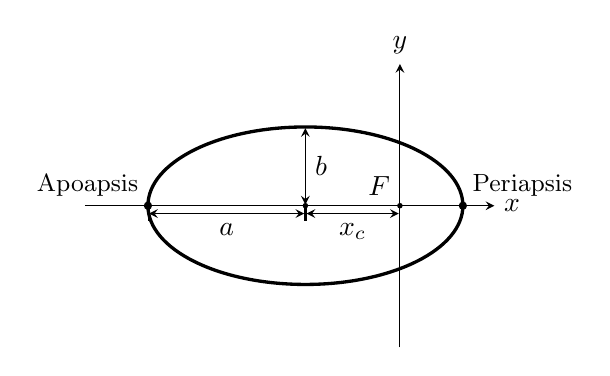
\begin{tikzpicture}[>=stealth]
  \draw[->] (0, -1.8) -- (0, 1.8) node[above] {$y$};
  \draw[->] (-4, 0) -- (1.2, 0) node[right] {$x$};

  \begin{scope}[xshift=-1.2cm]
    \draw[very thick] (0, 0) ellipse (2cm and 1cm);
    \draw[|<->|] (0, -0.1) -- (1.2cm, -0.1) node[midway, below] {$x_c$};
    \draw[|<->|] (0, 0) -- (0, 1) node[midway, right] {$b$};
    \draw[|<->|] (0, -0.1) -- (-2cm, -0.1) node[midway, below] {$a$};
    \fill (0, 0) circle (1pt);
    \fill (1.2, 0) circle (1pt) node[above left] {$F$};
    \fill (2cm, 0) circle (1.5pt) node[above right] {\small Periapsis};
    \fill (-2cm, 0) circle (1.5pt) node[above left] {\small Apoapsis};
  \end{scope}
\end{tikzpicture}
\end{center}
The body the object is orbiting is at the focus $F$ as this corresponds to $r = 0$.
\subsubsection{Parabolic Orbit -- $e = 1$}
We see that this is unbounded as the denominator of \cref{keplerProblem} can be 0.
Setting $e = 1$, we have the Cartesian equation:
\begin{align*}
  (r^2_0 - x)^2 &= x^2 + y^2 \\
  r^2_0 - 2r_0 x + \cancel{x^2} &= \cancel{x^2} + y^2 \\
  y^2 &= - 4\left(\frac{r_0}{2}\right)\left(x - \frac{r_0}{2}\right) \\
      &= -4a(x - x_c)
\end{align*}
which is a parabola.
\begin{center}
\begin{tikzpicture}[>=stealth]
  \draw[->] (0, -2) -- (0, 2) node[above] {$y$};
  \draw[->] (-3, 0) -- (1.8, 0) node[right] {$x$};

  \fill (1.2cm, 0) circle (1.5pt) node[above right] {\small Periapsis};

  \draw[|<->|] (0, -0.1) -- (1.2cm, -0.1) node[midway, below] {$x_c$};
  \clip (-3, -3) rectangle (3, 3);
  \begin{scope}[xshift=1.2cm]
    \draw[very thick, rotate=90,domain=-2:2, samples=50] plot ({\x}, {(\x)^2});

    \fill (-1.2, 0) circle (1pt) node[above left] {$F$};
  \end{scope}
\end{tikzpicture}
\end{center}
\subsubsection{Hyperbolic Orbit -- $e > 1$}
We see that this is unbounded again.
$r \to \infty$ at $\cos \theta = - \frac{1}{e}$ so we get two asymptotes.

Deriving the Cartesian equation is almost identical to with the ellipse, however as $e > 1$, $1 - e^2 < 0$, we define $b^2 = - \frac{r^2_0}{(1 - e^2)^3}$, yielding:
\[
  \frac{(x - x_c)^2}{a^2} - \frac{y^2}{b^2} = 1
\]
which is a hyperbola.
\begin{center}
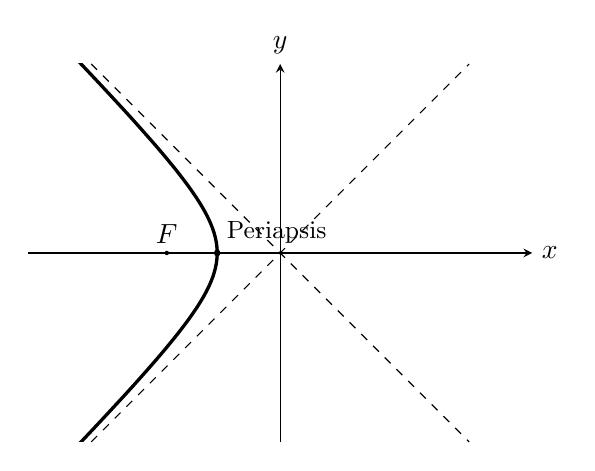
\begin{tikzpicture}[>=stealth, scale=0.8]
  \draw[->] (0, -3) -- (0, 3) node[above] {$y$};
  \draw[->] (-4, 0) -- (4, 0) node[right] {$x$};

  \fill (-1cm, 0) circle (1.5pt) node[above right] {\small Periapsis};
  \begin{scope}
    \clip (-4, -3) rectangle (4, 3);
    \draw[very thick, rotate=180, domain=-1.4:1.4, smooth, variable=\t] plot ({sec(\t r)},{tan(\t r)});
  \end{scope}

  \draw[dashed] (-3, -3) -- (3, 3);
  \draw[dashed] (-3, 3) -- (3, -3);

  \fill (-1.8, 0) circle (1pt) node[above] {$F$};
\end{tikzpicture}
\end{center}

\subsection{Energy of Solutions}
\label{keplerEnergy}
There are many results relating to conic sections, which can all be derived using formulae above (see Example Sheet 2).
Using the solved form is not always the best way to derive a result, using the conservation of energy often leads to a more elegant solution.

We can evaluate the energy of the solutions we found in the previous section:
\begin{align*}
  E &= \frac{1}{2}m \dot{r}^2 + \frac{m\ell^2}{2r^2} - \frac{km}{r} \\
    &= \frac{1}{2}m \ell^2 \left(\deriv{u}{\theta}\right)^2 + \frac{1}{2} m\ell^2 u^2 - kmu \text{ as $\dot{r} = -\ell \deriv{u}{\theta}$ and $\frac{1}{r} = u$} \\
    &= \frac{1}{2}m \ell^2 \left(\frac{k^2e^2}{\ell^4} \sin^2 \theta\right) + \frac{1}{2} m\ell^2 \left(\frac{k e}{\ell^2} \cos \theta + \frac{k}{\ell^2}\right)^2 - km\left(\frac{ke}{\ell^2}\cos\theta + \frac{k}{\ell^2}\right) \\
    &= \frac{m k^2}{2\ell^2}e^2 + \frac{m k^2}{2\ell^2} - \frac{mk^2}{\ell^2} \\
    &= \frac{mk^2}{2\ell^2} (e^2 - 1)
\end{align*}
which is consistent with the energy associated with each orbit.
In particular, when $e = 0$, this is the minimum of $V_{\text{eff}}$, as we expect for a circular orbit.
\section{Kepler's Laws}
A consequence of the above are \textit{Kepler's laws of planetary motion}.
\begin{law}[Kepler's 1st Law]
  Each planet moves in an ellipse with the Sun at one focus.
\end{law}
\begin{proof}
  As shown in \cref{orbitTrajectories}.
\end{proof}
\begin{law}[Kepler's 2nd Law]
  The line between a planet and the Sun sweeps out equal areas in equal times.
\end{law}
\begin{proof}
  \begin{center}
  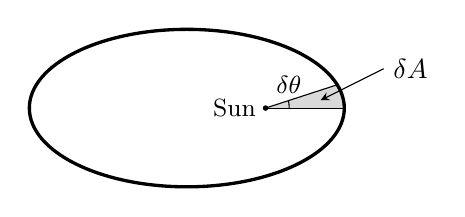
\begin{tikzpicture}[>=stealth]
    \fill (1, 0) circle (1pt) node[left] {\small Sun};
    \coordinate (A) at (1.91, 0.296);
    \coordinate (B) at (2, 0);
    \coordinate (C) at (2, 0.296);
    \begin{scope}
      \clip (0, 0) ellipse (2cm and 1cm);
      \fill[gray!30] (1, 0) -- (A) -- (C) -- (B) -- cycle;
    \end{scope}
    \draw[->] (2.5, 0.5) node[right] {$\delta A$} -- (1.7, 0.1);
    \draw[very thick] (0, 0) ellipse (2cm and 1cm);
    \draw (1, 0) -- (A);
    \draw (1, 0) -- (B);
    \draw (1.3,0) arc [start angle=0,end angle=10,radius=0.5] node[pos=0.7,above] {\small$\delta\theta$};
  \end{tikzpicture}
  \end{center}
  \[
    \delta A \approx \frac{1}{2}r^2 \delta \theta \implies \dot{A} = \frac{1}{2}r^2 \dot{\theta} = \frac{\ell}{2}
  \]
  which is a constant.
\end{proof}
\begin{remark}
  This only used the conservation of angular momentum and so holds for \textbf{any} central force.
\end{remark}
\begin{law}[Kepler's 3rd Law]
  The period of the orbit is proportional to $\text{radius}^{3/2}$.
\end{law}
It is natural for us to use dimensional analysis for this as we just need to show that it is proportional, not find any coefficients.
\begin{proof}[Dimensional Analysis]
  The only parameter in Newton's equation is $k = GM$ as the mass $m$ cancels on both sides.
  Therefore we can write $T = cR^{A}k^{B}$ for some coefficient $c$.
  $\frac{km}{r^2}$ is a force so we can find the units of $k$ as:
  \[
    \frac{[k]M}{L^2} = [F] = MLT^{-2} \implies [k] = L^3T^{-2}
  \]
  We can then equate units for $T$:
  \begin{align*}
    T = [T] &= [R]^{A}[k]^{B} \\
            &= L^{A}L^{3B}T^{-2B}
  \end{align*}
  Solving, we have $B = -\frac{1}{2}$ and $A = \frac{3}{2}$, so:
  \[
    T = c \frac{R^{\frac{3}{2}}}{k^{\frac{1}{2}}} \implies T \propto R^{\frac{3}{2}}
  \]
  as required.
\end{proof}
\begin{remark}[Notes]
  \begin{itemize}
    \item There is no unique radius associated to an ellipse but since we just require proportionality, any radius of the ellipse works.
    \item Kepler's 3rd law requires an inverse square force and so does not work with every central force.
  \end{itemize}
\end{remark}
We can also find the coefficient, provided that we exactly specify which radius we are using.
\begin{proof}
  Starting from Kepler's 2nd Law:
  \[
    \dot{A} = \frac{\ell}{2}
  \]
  A full period is therefore the area of the ellipse:
  \[
    T = \int_{0}^{T}  \d{t} = \int_{0}^{A_e} \frac{2}{\ell} \d{A} = \frac{2}{\ell}A_e
  \]
  where $A_e$ is the area of the ellipse.

  Recall from \cref{rMinMax} that for an elliptical orbit, $a^2 = \frac{r^2_0}{(1 - e^2)^2}$ and $b^2 = \frac{r^2_0}{(1 - e^2)}$.
  The area of an ellipse is $\pi ab$ so:
  \[
    A_e = \pi ab = \pi\frac{r^2_0}{(1 - e^2)^{3/2}}
  \]
  We defined $r_0 = \ell^2/k  \implies \ell = \sqrt{GMr_0}$ so:
  \[
    T = \frac{2}{\ell}A_e = \frac{2\pi}{\sqrt{GM}}\left[\frac{r_0}{(1 - e^2)}\right]^{\frac{3}{2}} = \frac{2\pi}{\sqrt{GM}}R^{\frac{3}{2}}_{\text{av}}
  \]
  where $R_{\text{av}}$ is the average radius as:
  \begin{align*}
    R_{\text{av}} &= \frac{r_0}{(1 - e^2)} \\
                  &= \frac{1}{2}\left(\frac{r_0}{1 + e} + \frac{r_0}{1 - e}\right) \\
                  &= \frac{1}{2}(r_{\text{min}} + r_{\text{max}})
  \end{align*}
  where $r_{\text{min}}$ and $r_{\text{max}}$ are from \cref{rMinMax}.
\end{proof}
\section{Repulsive Potentials and Scattering}
\subsection{Impact Parameter}
Given a central potential $V(r)$ such that $V \to 0$ as $r \to \infty$, one can perform \textit{scattering experiments}.
This is when we shoot in a particle from a large $r$ and see how it flies out again.
One important concept for this is the \textit{impact parameter}.
\begin{definition}[Impact Paramter]
  The \textit{impact parameter} $b$ is defined to be the closet the particle would have come to the target in the absence of any forces.
\end{definition}
\begin{center}
\begin{tikzpicture}[>=stealth, scale=1.2]
  \node[left] at (4.5, 1.2) {\tiny Interacting Trajectory};
  \draw[dashed, ->] (-4, 0) -- (4, 0) node[above left] {\tiny Non-interacting Trajectory};
  \fill (0, -0.7) circle (1.5pt) node[below] {Target};
  \draw (0, 0) -- (0, -0.7) node[midway, right] {$b$};
  \draw[very thick, postaction={decorate}, decoration={
          markings,
          mark=at position 0.2 with {\arrow{>}},
          mark=at position 0.4 with {\arrow{>}},
          mark=at position 0.6 with {\arrow{>}},
          mark=at position 0.8 with {\arrow{>}},
        }] plot [smooth, tension=0.5] coordinates { (-4, 0) (-3, 0) (-2, 0.1) (0, 0.6) (2, 1.3) };
\end{tikzpicture}
\end{center}
The impact parameter is related to the angular momentum $\ell$ by:
\[
  \ell = bv
\]
Consider first the non-interacting particle.
At the point closest, the velocity of the particle, $\dot{\vec{x}}$, and the position vector between the particle and the target (as the target it the origin), $\vec{x}$, are orthogonal so the angular momentum is $\ell = |\vec{x} \cdot \dot{\vec{x}}| = |\vec{x}| |\dot{\vec{x}}| = bv$.
The non-interacting particle has a conserved angular momentum and constant velocity so at all points $\ell = bv$.
So if we go very far back in the non-interacting particle's path, $\ell = bv$ still holds.

Now thinking about the interacting particle, the initial angular momentum $\ell$ is the same for the interacting and non-interacting particles because they both start far away from the target with the same velocity.
The interacting case also has a conserved angular momentum (as it only experiences a central force, see \cref{angularConserved}) and so always has $\ell = bv$.
\subsection{Rutherford Scattering}
Rutherford showed that certain scattering experiments of atoms could be explained if all the positive charge of the atom was contained in the nucleus.

Scattering by a \textbf{repulsive interaction} for two positively charged particles has the potential:
\[
  V(r) = \frac{\kappa}{r} \text{ where } \kappa = \frac{qQ}{4\pi\varepsilon_0}
\]
This is the potential for the Coulomb force from \cref{electricForces}.

We can reuse the results from the Kepler problem by mapping $-km \mapsto \kappa$.
In the Kepler problem, $r_0 = \frac{\ell^2}{k} \mapsto \widetilde{r}_0 = -\frac{\ell^2m}{\kappa}$ so:
\[
  r = \frac{\widetilde{r}_0}{\widetilde{e} \cos \theta - 1}
\]
where $\widetilde{r}_0 = \frac{\ell^2 m}{\kappa}$ and $\widetilde{e} = -e$.

We wish to find the angle $\phi$ through which the particle is scattered, as seen below:
\begin{center}
\begin{tikzpicture}[>=stealth, scale=1.3]
  \draw[dotted] (-4, 0) -- (4, 0) node[right] {$\theta = 0$};

  \fill (-1, 0) circle (1.5pt) node[above left] {\small Target};
  \begin{scope}
    \clip (-4, -3) rectangle (4, 3);
    \draw[very thick, domain=-1.4:1.4, smooth, variable=\t, postaction={decorate}, decoration={
          markings,
          mark=at position 0.4 with {\arrow{<}},
          mark=at position 0.6 with {\arrow{<}},
        }] plot ({sec(\t r)},{tan(\t r)});
  \end{scope}

  \draw (-0.354, -0.354) arc [start angle=-135,end angle=-45,radius=0.5] node[midway, below] {$\phi$};
  \draw (-0.354, 0.354) arc [start angle=135,end angle=45,radius=0.5] node[midway, above] {$\phi$};
  \draw (0.4, 0) arc [start angle=0,end angle=45,radius=0.4] node[midway, right] {$\alpha$};
  \draw (0.4, 0) arc [start angle=0,end angle=-45,radius=0.4] node[midway, right] {$\alpha$};

  \draw (-1, 0) -- (-0.5, -0.5) node[midway, below left] {$b$};
  \draw (-1, 0) -- (-0.5, 0.5) node[midway, above left] {$b$};

  \node at (0, -1.2) {\tiny Scattering Angle};

  \draw[dashed] (-3, -3) -- (3, 3);
  \draw[dashed] (-3, 3) -- (3, -3);
\end{tikzpicture}
\end{center}
Energy is conserved so the incoming velocity has the same magnitude as the outgoing velocity.
Since angular momentum is also conserved, the impact parameters for a particle from the incoming direction and for a particle from the outgoing direction.
This gives rise to the symmetry in the diagram above.

Using this symmetry, we have that $\pi = \phi + 2\alpha$.
Furthermore, since $\alpha$ is the angle with which $r \to \infty$, $\alpha$ satisfies $\widetilde{e}\cos \alpha = 1$ so that the denominator vanishes.

The initial and final energies of the particle are $E = \frac{1}{2}mv^2$ since $V \to 0$ as $r \to \infty$.
Then, using conservation of energy and the energy of solutions to the Kepler problem found in \cref{keplerEnergy}, we have:
\begin{align*}
  E = \frac{1}{2}mv^2 &= \frac{\kappa^2}{2\ell^2 m}(\widetilde{e}^2 - 1) \\
                      &= \frac{\kappa^2}{2mb^2v^2}(\sec^2\alpha - 1) \\
                      &= \frac{\kappa^2}{2mb^2v^2}\tan^2\alpha
\end{align*}
We can rewrite $\tan \alpha = \tan(\frac{\pi - \phi}{2}) = \frac{\sin(\pi/2 - \phi/2)}{\cos(\pi/2 - \phi/2)} = \frac{1}{\tan(\phi/2)}$ so:
\[
  E = \frac{1}{2}mv^2 = \frac{\kappa^2}{2mb^2v^2}\frac{1}{\tan^2(\phi/2)}
\]
Rearranging for $\phi$, we have:
\begin{align*}
  \tan^2(\phi/2) &= \frac{\kappa^2}{m^2b^2v^4} \\
  \implies \phi &= 2 \arctan\left(\frac{\kappa}{bmv^2}\right)
\end{align*}
For paths where the non-interacting trajectory would pass very close to the target, the impact parameter is very small and so we get large scattering angles.
This allows us to use scattering to find subatomic distances by measuring relatively large $\phi$ and then finding $b$.
\end{document}
